\documentclass[aspectratio=169]{beamer}
\usetheme{Madrid}
\usecolortheme{beaver}
\usepackage[utf8]{inputenc}
\usepackage[T1]{fontenc}
\usepackage{tikz}
\usepackage{amssymb}
\usepackage{graphicx}
\setbeamertemplate{navigation symbols}{}
\setbeamercolor{title}{fg=white,bg=cyan!60!black}
\setbeamercolor{frametitle}{fg=white,bg=cyan!50!black}
\setbeamercolor{block title}{bg=cyan!15,fg=black}
\setbeamercolor{block body}{bg=cyan!5,fg=black}

\title{G8 — Smart NPCs}
\subtitle{BOSS: Enemy with 3 Behaviours}
\author{ByteForge --- Grade 7 --- Game Maker}
\date{}

\begin{document}

\begin{frame}
    \titlepage
\end{frame}

\begin{frame}{BOSS — rules vs. real machine learning}
    \Large
    Every behaviour here is a rule YOU wrote. Real ML is different: instead of a human writing rules, the system is shown examples and works out its OWN rules.

    \begin{center}
    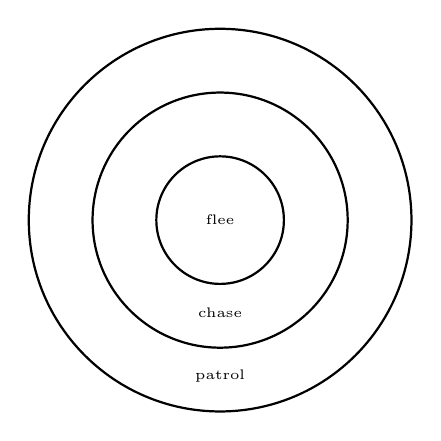
\begin{tikzpicture}[scale=0.9]

        \draw[thick] (0,0) circle (0.9);
        \draw[thick] (0,0) circle (1.8);
        \draw[thick] (0,0) circle (2.7);
        \node at (0,0) {\tiny flee};
        \node at (0,-1.3) {\tiny chase};
        \node at (0,-2.2) {\tiny patrol};
    \end{tikzpicture}
    \end{center}
\end{frame}

\begin{frame}{Your Turn}
    \Large
    Open the student map, find \textbf{G8 — Smart NPCs}, and complete
    the \textbf{BOSS} challenge --- everything you just saw, they now do themselves.
\end{frame}

\end{document}
